% Unified IR M2a — plan bundle
% Compile: pdflatex plan.tex
%
% plan.pdf is intentionally absent. The user granted an explicit plan.pdf
% tooling waiver on 2026-08-28 and directed that no TeX, Tectonic, Pandoc or
% other document toolchain be installed on this host. This bundle
% (.tex + .tikz + .mmd) is the reproducible source and is the deliverable.
% Recorded waiver, not an unmet §11 halt condition.

\documentclass[11pt,a4paper]{article}
\usepackage[T1]{fontenc}
\usepackage[utf8]{inputenc}
\usepackage[margin=25mm]{geometry}
\usepackage{booktabs}
\usepackage{longtable}
\usepackage{tikz}
\usetikzlibrary{positioning,fit,backgrounds,arrows.meta,calc}
\usepackage{hyperref}
\hypersetup{colorlinks=true,linkcolor=blue!50!black,urlcolor=blue!50!black}
\newcommand{\code}[1]{\texttt{#1}}

\title{Unified IR --- M2a\\[2pt]
       \large A storage-independent read surface for \code{hymeko\_core::ir::Ir}}
\author{HyMeKo framework}
\date{Created-at: \textbf{2026-08-28 21:41 CEST}}

\begin{document}
\maketitle

\begin{abstract}
\noindent
M2a is \textbf{additive only}. It adds the read boundary M2b migrates onto, so
that the M2d, M1 and M3 storage changes become invisible to call sites. No
existing field, method, type or storage is changed --- \code{ir/ir.rs} is not
edited at all, because inherent \code{impl} blocks may live in any module of the
defining crate.

\medskip
\noindent
Evidence: \code{reports/2026-08-28-unified-ir-m2a.md}. Migration table:
\code{docs/unified-ir-consumer-map.md}.
\end{abstract}

\section{Scope}

\paragraph{Goal.} One coherent read surface whose \emph{contracts} assume
nothing about storage: not dense ids, not ordinal stability, not the absence of
tombstones, not the existence of the parallel \code{decl\_to\_*} maps.
Implementations index ordinally \emph{inside} \code{Ir}; that is the boundary's
purpose.

\paragraph{Out of scope, deliberately.} Mutable accessors, \code{StableArena},
\code{IRDelta}, transactions, \code{Id<T>} changes, storage changes, making
fields private, parser/lowering, canonical hashes, hierarchy authority, sibling
repositories, HNN/WGPU, new dependencies.

\paragraph{Not built although the earlier stage sketch listed it.}
\code{push\_declaration}, which would consolidate the second lockstep writer in
\code{bridge.rs}, is a \emph{mutating} API and therefore outside M2a. It moves to
the first stage permitted to add mutation.

\section{The inventory came first, and changed the design}

Two requested capabilities already existed \emph{and were already safe}:

\begin{center}
\begin{tabular}{@{}lll@{}}
\toprule
\textbf{Requested} & \textbf{Existing} & \textbf{Action} \\
\midrule
\code{declaration(id)} & \code{Ir::decl\_node} & not added --- cosmetic rename \\
\code{node\_id\_for\_decl(id)} & \code{Ir::as\_node} \emph{et al.} & not added --- cosmetic rename \\
\bottomrule
\end{tabular}
\end{center}

\noindent
The repository's established term is \textbf{\code{decl}}, and the new surface
keeps it rather than introducing a second vocabulary.

\section{What is genuinely new}

Typed record lookup (\code{node}, \code{edge}, \code{arc}); declaration
$\rightarrow$ record with id and back-link verification
(\code{node\_for\_decl} \emph{et al.}); typed-id iterators (\code{decls},
\code{node\_records}, \code{edge\_records}, \code{arc\_records}); live-entity
counts; containment; and \textbf{total} hierarchy reads.

\paragraph{Totality is the substantive addition.} The pre-existing readers are
partial: \code{kind} and \code{decl\_kind} panic on \code{DeclId::NONE} --- a
value the type system hands out freely --- and \code{parent},
\code{first\_child}, \code{next\_sibling} and \code{decl\_children} panic on
out-of-range ids. Their signatures return \code{DeclId}/\code{DeclKind} rather
than \code{Option} and existing callers depend on that, so the total versions
are \emph{new} methods with an \code{\_of} suffix and the old ones are untouched.

\section{Test strategy}

\begin{description}\itemsep3pt
\item[Lookup] first/middle/last; \code{NONE}; exactly-past-the-end; a very large
  raw id; typed round-trip; raw ordinal 0 not aliasing across tables.
\item[Absence] a valid declaration lacking the requested record; a mapping
  naming a \emph{foreign} record; a mapping naming an out-of-range record. The
  middle case is the one that would otherwise be a silent wrong answer.
\item[Iteration] empty; singleton; counts equal iterator length; ids resolve
  back with no gaps or duplicates; repeated iteration stable. Order stability is
  asserted; order \emph{meaning} is not.
\item[Hierarchy] root, nested, siblings, leaf; child order identical to the
  existing iterator; termination on a sibling cycle.
\item[Compatibility] all 96 fixtures, gated on M0.6 coherence first: accessor
  versus direct field access, and new versus pre-existing helper, for every
  declaration.
\end{description}

\section{Performance --- measured, not asserted}

Variants are registered in \textbf{alternating rounds}, never as blocks.

\paragraph{The fair control.} Comparing \code{ir.decl\_nodes[d.0]} against
\code{ir.decl\_node(d)} is not like-for-like: the accessor additionally rejects
\code{NONE}, returns an \code{Option} and forces a branch. A third variant,
\code{direct\_guarded}, performs exactly that work by hand and is the honest
baseline.

\begin{center}
\begin{tabular}{@{}lrr@{}}
\toprule
\textbf{Variant (1\,500 declarations)} & \textbf{Median} & \textbf{vs control} \\
\midrule
\code{direct} (unguarded) & 538\,ns & --- \\
\code{direct\_guarded} (control) & \textbf{527\,ns} & baseline \\
\code{accessor} & 785\,ns & \textbf{+49\,\%} \\
\bottomrule
\end{tabular}
\end{center}

\noindent
The overhead \emph{survives} the fair control, so it is not the price of safety
but of materialising \code{Option<\&T>}. Absolute scale:
$\approx$0.35\,ns $\rightarrow$ $\approx$0.52\,ns per lookup. Iteration is
\textbf{within noise}. No allocation on any valid-lookup path; invalid lookup
remains O(1).

\paragraph{Verdict: REGRESSION, stated plainly.} Acceptance asked for
$<3\,\%$; that is not met for scalar lookup. Claiming otherwise would require
choosing a favourable framing.

\paragraph{A measurement-integrity finding.} The 10\,000-element case measured
16.5\,\textmu s and then 7.0\,\textmu s on identical benchmark code with
ambient load 2--4\,\% in both runs; the only change was a recompilation that
added a variant to the same group. This is \textbf{reported, not resolved} ---
attributing it would need generated-code inspection this phase may not install
tooling for --- and the conclusions rest on the 1\,000-element case, which was
stable across both runs.

\section{Rollback}

The entire phase is one new module plus one \code{pub mod} line. Reverting is a
single commit, and nothing depends on the new surface yet.

\section{Risk anticipation}

\paragraph{Performance-contract preservation.} No existing code path was
touched, so no existing contract can regress; the measured cost applies only to
\emph{new} call sites. M2b must therefore migrate reads on correctness grounds,
not on a performance promise --- and \code{canonical\_hash.rs} and
\code{hash\_pass.rs}, already inside the boundary, may keep indexing directly.

\paragraph{The hazard that is not here.} The accessors make \emph{reads}
storage-independent. Writes are not, and \code{bridge.rs} in
\code{transformation} remains a second writer of core's five-array lockstep.
M2a does not reduce that risk and must not be read as having done so.

\section{Hash debt, unchanged}

M2a changes no hash. \code{canonical\_program\_hash} v1 remains structural-only;
\code{bases} remains absent from both identity systems;
\code{compute\_merkle\_hashes} may still omit incidence targets under adverse id
order; serialized \code{decl\_hash} still carries no \code{algo\_version}.
Accessor work implies nothing about any of these.

\section{Figures}

% Unified IR M2a — accessor boundary (TikZ). Created-at: 2026-08-28 21:41 CEST
% % Unified IR M2a — accessor boundary (TikZ). Created-at: 2026-08-28 21:41 CEST
% % Unified IR M2a — accessor boundary (TikZ). Created-at: 2026-08-28 21:41 CEST
% \input{plan.tikz} from plan.tex, which supplies the preamble.
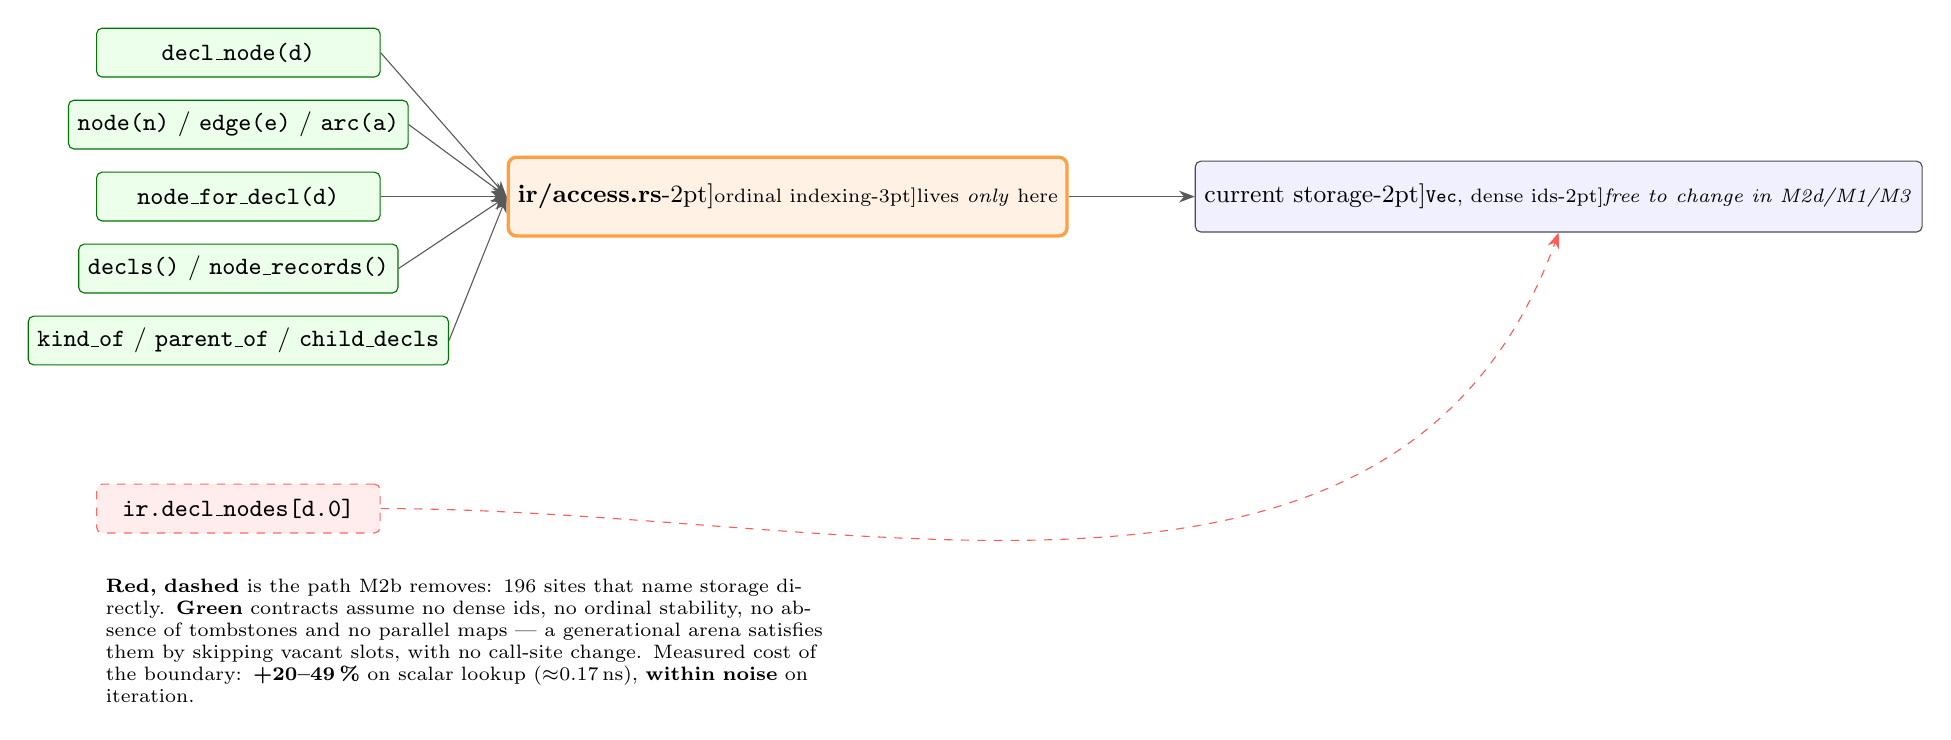
\begin{tikzpicture}[
    font=\small,
    api/.style={draw=green!45!black, fill=green!8, rounded corners=2pt,
                minimum width=3.6cm, minimum height=0.62cm, align=center},
    raw/.style={draw=red!60, fill=red!7, rounded corners=2pt, dashed,
                minimum width=3.6cm, minimum height=0.62cm, align=center},
    store/.style={draw=black!70, fill=blue!6, rounded corners=2pt,
                  minimum width=4.2cm, minimum height=0.9cm, align=center},
    bnd/.style={draw=orange!75, fill=orange!10, very thick, rounded corners=3pt,
                minimum width=4.6cm, minimum height=1.0cm, align=center},
    a/.style={-{Stealth[length=2mm]}, black!65},
    node distance=0.28cm and 1.6cm,
]
\node[api] (a1) {\texttt{decl\_node(d)}};
\node[api, below=of a1] (a2) {\texttt{node(n)} / \texttt{edge(e)} / \texttt{arc(a)}};
\node[api, below=of a2] (a3) {\texttt{node\_for\_decl(d)}};
\node[api, below=of a3] (a4) {\texttt{decls()} / \texttt{node\_records()}};
\node[api, below=of a4] (a5) {\texttt{kind\_of} / \texttt{parent\_of} / \texttt{child\_decls}};

\node[bnd, right=of a3] (b) {\textbf{ir/access.rs}\[-2pt]\scriptsize ordinal indexing\[-3pt]\scriptsize lives \emph{only} here};
\node[store, right=of b] (s) {current storage\[-2pt]\scriptsize \texttt{Vec}, dense ids\[-2pt]\scriptsize \emph{free to change in M2d/M1/M3}};

\foreach \x in {a1,a2,a3,a4,a5} \draw[a] (\x.east) -- (b.west);
\draw[a] (b) -- (s);

\node[raw, below=1.5cm of a5] (r) {\texttt{ir.decl\_nodes[d.0]}};
\draw[a, red!65, dashed] (r.east) to[out=0,in=250] (s.south);

\node[align=left, anchor=north west, font=\scriptsize, text width=9.2cm]
      at ($(r.south west)+(0,-0.45)$)
      {\textbf{Red, dashed} is the path M2b removes: 196 sites that name storage
       directly. \textbf{Green} contracts assume no dense ids, no ordinal
       stability, no absence of tombstones and no parallel maps --- a
       generational arena satisfies them by skipping vacant slots, with no
       call-site change. Measured cost of the boundary: \textbf{+20--49\,\%} on
       scalar lookup ($\approx$0.17\,ns), \textbf{within noise} on iteration.};
\end{tikzpicture}
 from plan.tex, which supplies the preamble.
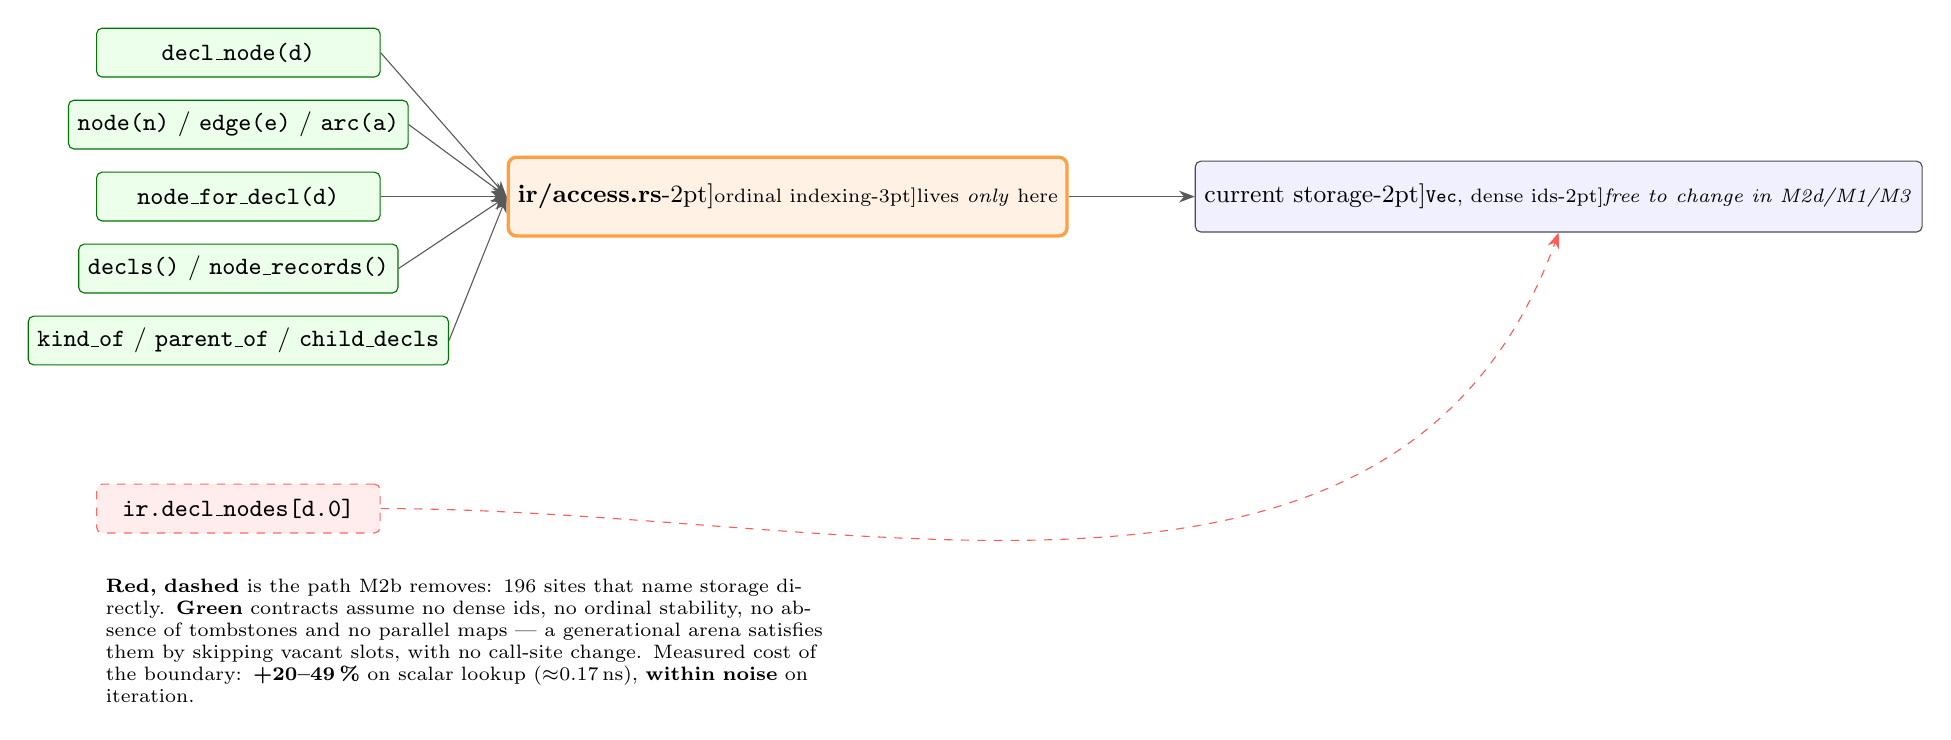
\begin{tikzpicture}[
    font=\small,
    api/.style={draw=green!45!black, fill=green!8, rounded corners=2pt,
                minimum width=3.6cm, minimum height=0.62cm, align=center},
    raw/.style={draw=red!60, fill=red!7, rounded corners=2pt, dashed,
                minimum width=3.6cm, minimum height=0.62cm, align=center},
    store/.style={draw=black!70, fill=blue!6, rounded corners=2pt,
                  minimum width=4.2cm, minimum height=0.9cm, align=center},
    bnd/.style={draw=orange!75, fill=orange!10, very thick, rounded corners=3pt,
                minimum width=4.6cm, minimum height=1.0cm, align=center},
    a/.style={-{Stealth[length=2mm]}, black!65},
    node distance=0.28cm and 1.6cm,
]
\node[api] (a1) {\texttt{decl\_node(d)}};
\node[api, below=of a1] (a2) {\texttt{node(n)} / \texttt{edge(e)} / \texttt{arc(a)}};
\node[api, below=of a2] (a3) {\texttt{node\_for\_decl(d)}};
\node[api, below=of a3] (a4) {\texttt{decls()} / \texttt{node\_records()}};
\node[api, below=of a4] (a5) {\texttt{kind\_of} / \texttt{parent\_of} / \texttt{child\_decls}};

\node[bnd, right=of a3] (b) {\textbf{ir/access.rs}\[-2pt]\scriptsize ordinal indexing\[-3pt]\scriptsize lives \emph{only} here};
\node[store, right=of b] (s) {current storage\[-2pt]\scriptsize \texttt{Vec}, dense ids\[-2pt]\scriptsize \emph{free to change in M2d/M1/M3}};

\foreach \x in {a1,a2,a3,a4,a5} \draw[a] (\x.east) -- (b.west);
\draw[a] (b) -- (s);

\node[raw, below=1.5cm of a5] (r) {\texttt{ir.decl\_nodes[d.0]}};
\draw[a, red!65, dashed] (r.east) to[out=0,in=250] (s.south);

\node[align=left, anchor=north west, font=\scriptsize, text width=9.2cm]
      at ($(r.south west)+(0,-0.45)$)
      {\textbf{Red, dashed} is the path M2b removes: 196 sites that name storage
       directly. \textbf{Green} contracts assume no dense ids, no ordinal
       stability, no absence of tombstones and no parallel maps --- a
       generational arena satisfies them by skipping vacant slots, with no
       call-site change. Measured cost of the boundary: \textbf{+20--49\,\%} on
       scalar lookup ($\approx$0.17\,ns), \textbf{within noise} on iteration.};
\end{tikzpicture}
 from plan.tex, which supplies the preamble.
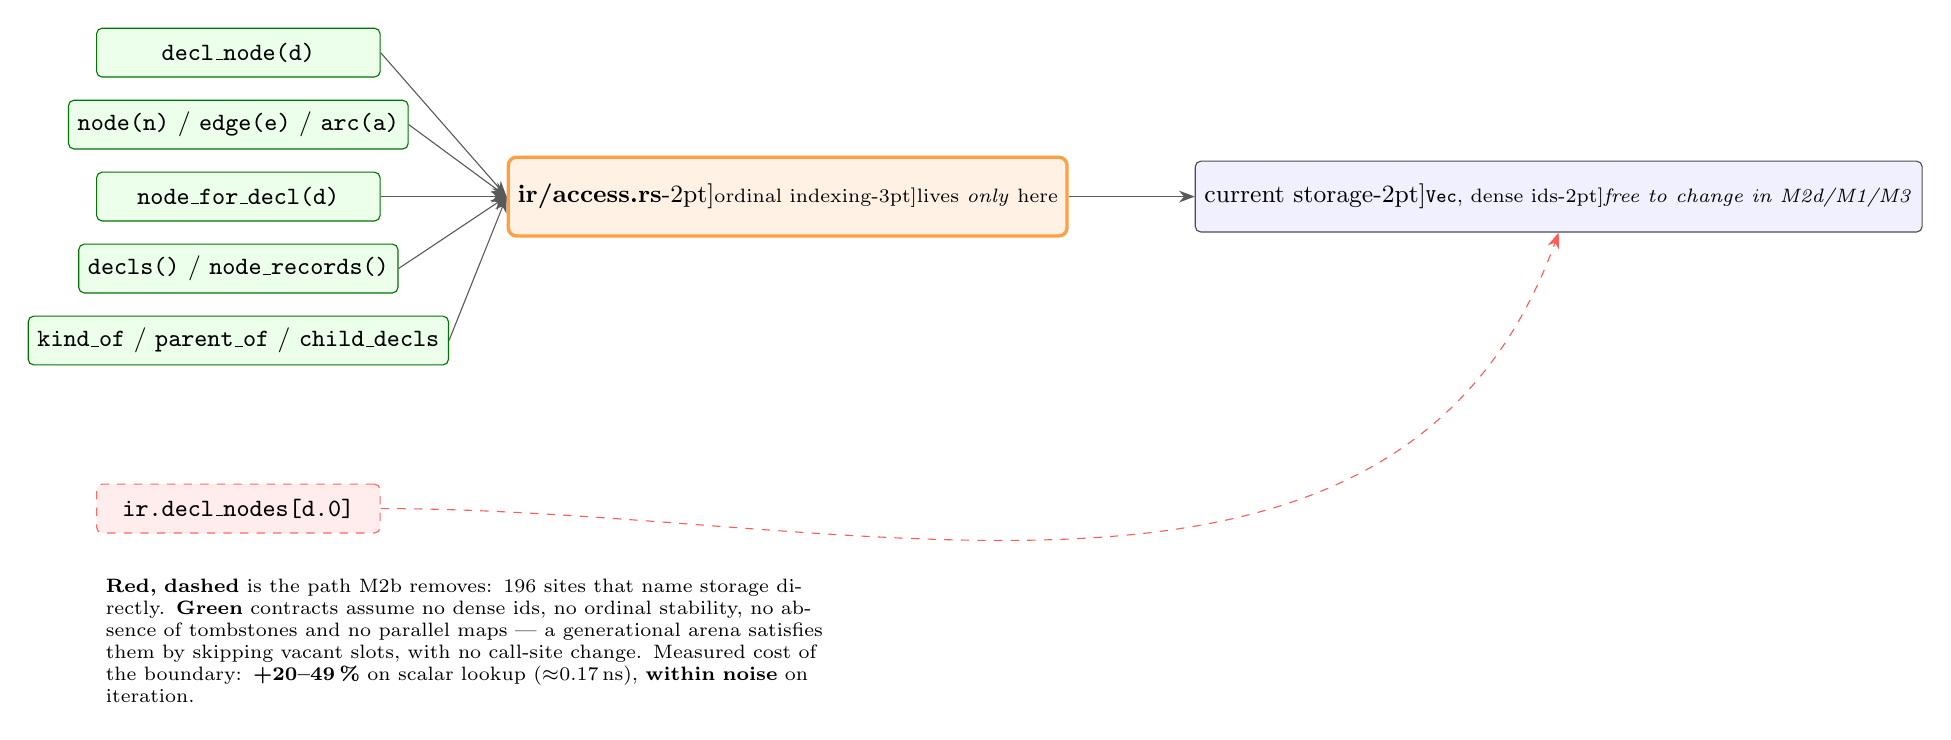
\begin{tikzpicture}[
    font=\small,
    api/.style={draw=green!45!black, fill=green!8, rounded corners=2pt,
                minimum width=3.6cm, minimum height=0.62cm, align=center},
    raw/.style={draw=red!60, fill=red!7, rounded corners=2pt, dashed,
                minimum width=3.6cm, minimum height=0.62cm, align=center},
    store/.style={draw=black!70, fill=blue!6, rounded corners=2pt,
                  minimum width=4.2cm, minimum height=0.9cm, align=center},
    bnd/.style={draw=orange!75, fill=orange!10, very thick, rounded corners=3pt,
                minimum width=4.6cm, minimum height=1.0cm, align=center},
    a/.style={-{Stealth[length=2mm]}, black!65},
    node distance=0.28cm and 1.6cm,
]
\node[api] (a1) {\texttt{decl\_node(d)}};
\node[api, below=of a1] (a2) {\texttt{node(n)} / \texttt{edge(e)} / \texttt{arc(a)}};
\node[api, below=of a2] (a3) {\texttt{node\_for\_decl(d)}};
\node[api, below=of a3] (a4) {\texttt{decls()} / \texttt{node\_records()}};
\node[api, below=of a4] (a5) {\texttt{kind\_of} / \texttt{parent\_of} / \texttt{child\_decls}};

\node[bnd, right=of a3] (b) {\textbf{ir/access.rs}\[-2pt]\scriptsize ordinal indexing\[-3pt]\scriptsize lives \emph{only} here};
\node[store, right=of b] (s) {current storage\[-2pt]\scriptsize \texttt{Vec}, dense ids\[-2pt]\scriptsize \emph{free to change in M2d/M1/M3}};

\foreach \x in {a1,a2,a3,a4,a5} \draw[a] (\x.east) -- (b.west);
\draw[a] (b) -- (s);

\node[raw, below=1.5cm of a5] (r) {\texttt{ir.decl\_nodes[d.0]}};
\draw[a, red!65, dashed] (r.east) to[out=0,in=250] (s.south);

\node[align=left, anchor=north west, font=\scriptsize, text width=9.2cm]
      at ($(r.south west)+(0,-0.45)$)
      {\textbf{Red, dashed} is the path M2b removes: 196 sites that name storage
       directly. \textbf{Green} contracts assume no dense ids, no ordinal
       stability, no absence of tombstones and no parallel maps --- a
       generational arena satisfies them by skipping vacant slots, with no
       call-site change. Measured cost of the boundary: \textbf{+20--49\,\%} on
       scalar lookup ($\approx$0.17\,ns), \textbf{within noise} on iteration.};
\end{tikzpicture}


\noindent
Boundary and totality views are in \code{plan.mmd}.

\end{document}
